% This is based on the LLNCS.DEM the demonstration file of % the LaTeX macro
% package from Springer-Verlag % for Lecture Notes in Computer Science, version
% 2.4 for LaTeX2e as of 16. April 2010
%
% See http://www.springer.com/computer/lncs/lncs+authors?SGWID=0-40209-0-0-0
% for the full guidelines.
\documentclass{llncs}
\usepackage{graphicx}
\graphicspath{ {./assets/} }

\usepackage{enumitem}
\setlist[enumerate]{itemsep=2mm}

\usepackage{dirtytalk}
\usepackage{minted}
\usepackage{amsmath}
\usepackage{pdflscape}
\usepackage[pass]{geometry}

%
% Tables
% --------
\usepackage[table]{xcolor}
\usepackage{hhline}
\usepackage{booktabs} % much better tables
\usepackage{multirow} % allows to fuse rows
\usepackage{array}    % manipulate array
\usepackage{tabularx} % better tables

% Define new tabularx column types:
%  - R: streteched right aligned
%  - C: stretched centered
%  - N: left aligned, specified space
\newcolumntype{R}{>{\raggedleft\arraybackslash}X}
\newcolumntype{C}{>{\centering\arraybackslash}X}
\newcolumntype{N}[1]{>{\raggedleft\arraybackslash}p{#1}}
\newcolumntype{S}{>{\hsize=.5\hsize}C}

% Set row height multiplicator to provide more breathing space
\renewcommand{\arraystretch}{1.5}

\usepackage[backend=biber]{biblatex}
\addbibresource{bibliography.bib}

\pagestyle{plain}
\setcounter{page}{1}
\pagenumbering{arabic}

\usepackage{pgfplots}
\pgfplotsset{width=6cm}
\usepackage{float}
\usepackage[caption = false]{subfig}

\begin{document}

\title{Multi-client Partially Non-Interactive and Instantaneous One-way Payment Channel for Ethereum}
\author{Thomas Shababi\inst{1} \and Jo\"el Gugger\inst{1} \and Daniel Lebrecht\inst{1}}

\authorrunning{Thomas~S.~Shababi et al.}
\tocauthor{Thomas~S.~Shababi, Joel Gugger, and Daniel Lebrecht}
\subtitle{{\normalsize\today{\small\ -- DRAFT}}}
\institute{TrueLevel SA, Neuch\^atel, Switzerland\\ \email{\{tom, joel, d\}@truelevel.io}}

\maketitle

\begin{abstract} Ethereum is a distributed computing platform and operating system featuring smart contract functionality. Transactions are faster than many other blockchains but not instant and each of them cost some ``gas''. This gas is used to quantify the amount of fee to pay for computation. \keywords{Crypto-currencies, Ethereum, Payment channels}
\end{abstract}

\section{Introduction}

\subsubsection{Requirements Language}
The key words ``MUST", ``MUST NOT", ``REQUIRED", ``SHALL", ``SHALL NOT",
``SHOULD", ``SHOULD NOT", ``RECOMMENDED", ``MAY", and ``OPTIONAL" in this
document are to be interpreted as described in RFC 2119 \cite{Bradner1997}.

\section{Multi-clients payment channels} Partially non-interactive multi-clients payment channels are composed of clients $c \in \mathcal{C}$ and one provider $\mathcal{P}$. $\mathcal{C}$ is the set of all clients registered in the multi-clients payment channel. Clients can send money to the provider through the channel but cannot receive through the channel.

A payment channel is by definition a structure composed of two layers of states. The first layer of states is registered on the blockchain, i.e. ``on-chain'' or contract states $\mu \in M$, and the second layer of states is kept ``off-chain'' between the participants and the provider, i.e. channel states $\sigma \in \Sigma$. States are sets of deltas. A delta represents an atomic change in a state. Delta changes $\delta \in \Delta$ are used to transition from one state to another.

We denote a main channel $\omega \in \Omega$ and assume the existence of sub-channels. The main channel $\omega$ is composed of two layers previously defined $(\Sigma, M)$.

Each client have a pair of states $(\mu_c, \sigma_c)$ shared with the provider. Only the latest pair is relevant, for each transition the new state in $\Sigma$ or $M$ is kept. We denote $\mu_c$ and $\sigma_c$ the contract and channel states for a client $c \in \mathcal{C}$. Hereinafter it is implied that all $\mu, \sigma$ correspond to one specific and only one client at any given time, but we forget $c$ to simplify the notation.

Transition from one state to another is denoted with $\rightarrow$, e.g. $\sigma \rightarrow \sigma'$ or $\mu \rightarrow \mu'$. Transitions in $\Sigma$ depend on particular deltas in $\Delta_\sigma$ noted $\delta_\sigma$. We denote a transition from $\sigma, \sigma' \in \Sigma$ that depends on $\delta_\sigma \in \Delta_\sigma$ as
$$\sigma \xrightarrow{\delta_\sigma} \sigma'$$

And transitions in $M$ depending on particular deltas in $\Delta_\mu$ noted $\delta_\mu$ as
$$\mu \xrightarrow{\delta_\mu} \mu'$$

Transitivity law is applied on transitions. If there exists a transition from a state $s$ to another state $s'$ that depends on $t$ and $s'$ to $s''$ depending on $t'$, then there exists a transition from $s$ to $s''$ as
$$s \xrightarrow{t} s' \land s' \xrightarrow{t'} s'' \implies s \xrightarrow{t + t'} s''$$

We define predecessor and successor in states $\Sigma$ and $M$. If state $s$ is a predecessor of $s'$ we denote them as $s \prec s'$, or $s'$ is a successor of $s$ as $s' \succ s$. We denote the latest transition of a certain type as $\lceil \xrightarrow{t} \rceil$.

Layers are linked together, changes in contract layer affect the channel layer and the channel layer can be dictated, or applied, on the contract layer. We denote the application of $\sigma$ on $\mu$, i.e. dictate a channel state on the contract layer, also as $\sigma(\mu) = \mu'$. The full transition rule for contract states is defined as
$$\mu \xrightarrow{\delta_\mu \lor \sigma} \mu'$$

and the full transition rule for channel states as
$$\sigma \xrightarrow{\delta_\sigma \lor \mu \rightarrow \mu'} \sigma'$$

We can notice that each transition in contract states $M$ triggers a transition in channel states $\Sigma$. States are represented as sets of deltas $\delta \in \Delta$. We define how to compute the resulting state.
\begin{equation*}
\begin{split}
    \mu \xrightarrow{\delta_\mu} \mu' &: \quad \mu' = \mu \cup \{\delta_\mu\} \\
    \mu \xrightarrow{\sigma} \mu' &: \quad \mu' = \mu \cup \sigma \\
    \sigma \xrightarrow{\delta_\sigma} \sigma' &: \quad \sigma' = \sigma \cup \{ \delta_\sigma \}  \\
    \sigma \xrightarrow{\mu \xrightarrow{\delta_\mu} \mu'} \sigma' &: \quad \sigma' =  \sigma \cup \mu' = \sigma \cup \{ \delta_\mu \} \\
    \sigma \xrightarrow{\mu \xrightarrow{\sigma''} \mu'} \sigma' &: \quad \sigma' = \mu' \\
\end{split}
\end{equation*}

It is worth noting that the last rule $\sigma \xrightarrow{\mu \xrightarrow{\sigma''} \mu'} \sigma'$ has implications on the validity of deltas. Because the resulting channel state $\sigma'$ is equal to the contract state $\mu'$, all deltas $\delta_\sigma$ applied between the dictated state $\sigma''$ and the starting state $\sigma$, where $\sigma'' \preceq \sigma$, are discarded. If we have
\begin{equation*}
\begin{split}
    \Sigma&: \emptyset \xrightarrow{\emptyset \xrightarrow{\delta_\mu} \mu_1} \sigma_1 \xrightarrow{\delta_\sigma} \sigma_2 \xrightarrow{\delta_\sigma'} \sigma_3 \xrightarrow{\mu_1 \xrightarrow{\sigma_2} \mu_2} \sigma_4\\
    M&: \emptyset \xrightarrow{\delta_\mu} \mu_1 \xrightarrow{\sigma_2} \mu_2 \\
\end{split}
\end{equation*}

we can see that a channel state $\sigma$ can be dictated on a contract state $\mu$ if the channel state is a successor of the latest updated state
$$\sigma(\mu) \iff \sigma \succ \sigma'' : \sigma' \lceil \xrightarrow{\mu \xrightarrow{\sigma'''} \mu'} \rceil \sigma''$$

%\begin{equation*}
%\begin{align*}
%    &\emptyset &\xrightarrow{\emptyset \xrightarrow{\delta_\mu} \mu_1}& &\sigma_1 &\xrightarrow{\delta_\sigma}& &\sigma_2 &\xrightarrow{\delta_\sigma'}& &\sigma_3 &\xrightarrow{\mu_1 \xrightarrow{\sigma_2} \mu_2}& &\sigma_4\\
%    &\emptyset &\xrightarrow{\delta_\mu}& &\mu_1 &\xrightarrow{\sigma_2}& && && && &\mu_2 \\
%\end{align*}
%\end{equation*}

We see that all channel states based on $\sigma_4$ will never contain $\delta_\sigma'$ because the dictated channel state used is $\sigma_2$ and not $\sigma_3$, then as soon as $\sigma_2$ is applied $\sigma_3$ becomes invalid by the previous rule.
\begin{align*}
    \mu_1    &= \emptyset \cup \{\delta_\mu\} & &= \{\delta_\mu\} \\
    \sigma_1 &= \emptyset \cup \{\delta_\mu\} & &= \{\delta_\mu\} \\
    \sigma_2 &= \{\delta_\mu\} \cup \{\delta_\sigma\} & &= \{\delta_\mu,\delta_\sigma\} \\
    \sigma_3 &= \{\delta_\mu,\delta_\sigma\}\cup\{\delta_\sigma'\} & &= \{\delta_\mu,\delta_\sigma,\delta_\sigma'\} \\
    \mu_2    &= \{\delta_\mu\} \cup \{\delta_\mu,\delta_\sigma\} & &= \{\delta_\mu,\delta_\sigma\} \\
    \sigma_4 &=  \{\delta_\mu,\delta_\sigma\} & &= \{\delta_\mu,\delta_\sigma\} \\
\end{align*}

%Contract state transitions are triggered by external events $e \in \mathcal{E}$ or messages $m \in \mathcal{M}$. Transitions between two states $\mu, \mu' \in M$ are denoted $\mu \rightarrow \mu '$. If the transition is due to an external event $e$ we write $\mu \xrightarrow{e} \mu '$. If the transition is due to a message $m$ we write $\mu \xrightarrow{m} \mu '$. Generic transitions are noted as $\mu \rightarrow \mu '$.
%
%A message $m$ can be ``applied'' to a state $\mu$, we denote this operation with $m(\mu)$, i.e. $\mu \xrightarrow{m} \mu'$. Messages are created based on a channel states. Each channel state $\sigma \in \Sigma$ can derive its corresponding message $m \in \mathcal{M}$
%$$\forall \sigma \in \Sigma,\ \exists m\ |\ m \in \mathcal{M}$$
%
%In reality it is not necessary to derive all messages. Some external events (e.g. top ups) afect the channel states that trigger transitions in $\Sigma$, but correspondig messages are only created when needed.

\section{Building blocks}
\subsection{Contract state variables} We define variables to acces the contract state $\mu \in M$ for a client $c \in \mathcal{C}$.

\subsubsection{Current validity index, $I_\mu$} For each client the current index $I_\mu$ must be retreivable, $\forall c \in \mathcal{C}, \quad \exists I_\mu \in \mu >= 0$. The index for a client must start from $0$.

\subsubsection{Current contract client balance, $B_\mu$} For each client the current contract balance amount must be retrievable, $\forall c \in \mathcal{C}, \quad \exists B_\mu \in \mu >= 0$. It is worth noting that this current contract balance is not the same as the current channel balance or, in other words, the remaining amount of a client in the channel.

\subsubsection{Current provider refund amount, $R_\mathcal{P}$} For each client the current provider refund amount must be retrievable, $\forall c \in \mathcal{C}, \quad \exists R_\mathcal{P} \in \mu$ such that $R_\mathcal{P}$ is the provider owned amount at the moment of the request. The remaining money must go to the client.

\subsection{Contract states} Each client $c \in \mathcal{C}$ in the contract is defined by an on-chain state $\mu_c \in M$. States $\mu \in M$ are represented as
$$\mu_c = (I_\mu, B_\mu, R_\mathcal{P})$$

\subsection{Channel state variables} We define variables to represent: (i) the lifetime of a single channel in the multi-clients channel architecture, (ii) the total amount deposited for a client over the lifetime, (iii) the total amount sent to the provider over the lifetime, and (iv) the minimal and full available amount for the client.

\subsubsection{Channel lifetime} It exists one lifetime and only one per element in $\mathcal{C} \times \mathcal{P}$ and begins when the first deposit is made, i.e. one lifetime per client $c \in \mathcal{C}$.

\subsubsection{Last observed validity index, $I_\sigma$} The last observed validity index is a copy of contract validity index at the moment where the state is created.

\subsubsection{Last observed client balance, $B_\sigma$} Same as the validity index but the client balance.

\subsubsection{Total deposit, $D$} Total deposit of a client represents the total amount recieved from the begining of the lifetime. Each top up increases the total deposit.

\subsubsection{Total spent, $S$} Total amount sent to the provider by a client represents the sum of all payments since the begining of the lifetime. Each payment increases the total spent.

\subsubsection{Client refunded amount, $R$} Total amount refunded to the client since the begining of the lifetime. Each refund can increase the total client refunded amount.

\subsubsection{Minimal available amount, $A_m$} Minimal amount available for a client is computed with the latest channel state $\sigma$. Without quering the contract state $\mu$ it is impossible to know if a bigger amount is now available. The minimal available amount is computed with
$$A_m = D - S - R$$

\subsubsection{Client available amount, $A$} The full amount available into a single channel for a client is computed with
$$A = D - S - R + B_\mu - B_\sigma, \quad B_\mu \geq A$$

It is worth noting that $B_\mu - B_\sigma$ is added to the difference of total deposit and total spent in case of new on-chain delta changes.

\subsection{Channel states} Each client $c \in \mathcal{C}$ is defined by their channel state $\sigma \in \Sigma$. States $\sigma \in \Sigma$ are composed of: (i) a validity index, (ii) the latest observed on-chain balance
of the client, (iii) the total deposit of the client, (iv) the total owned by the provider, and (v) the client total refunded amount. We denote a state $\sigma_c \in \Sigma$ as
$$\sigma_c = (I_\sigma, B_\sigma, D, S,R)$$

\subsection{Modifying channel states and contract states with Deltas} Deltas $\delta \in \Delta$ represent external channel capabilities of changing states $\Sigma$ and contract states $M$. Along with directives, they encapsulate all the channel capabilities. In this proposed channel architecture capabilities are: send money through the channel from clients to provider, create and top up a channel, settle a channel, and ask and get a refund. In that list, external capabilities are sending money through the channel, creating a channel, and top up a channel.

\subsubsection{Payment, $\delta_\sigma(a)$} This delta is used to increase the channel balance of the provider $O(\mathcal{P})$ of $a$ amount from a client $c$. Payment deltas are sent by clients to the provider. For each payment an acquired settle directive $d_s$ is generated by the client and sent to the provider.

\subsubsection{Top up, $\delta_\mu(a)$} This delta is used to increase the contract balance of a client by $a$ amount. Top up deltas are sent by anyone for any specific channel, i.e. client.

Creating channels is a special case of top up, when a channel is top up but does not already exists, the channel is created. The first delta of all channel will always be a top up.

\subsection{Dictate channel state on contract layer with Messages \& Directives} We define in the previous chapter a transition in contract layer performed with a channel state noted $\mu \xrightarrow{\sigma} \mu'$ or $\sigma(\mu) = \mu'$. These transitions are performed by the intermediary of messages $m \in \mathcal{M}$ and directives $d$.

Messages $m \in \mathcal{M}$ are an intermediary representation of channel states between the channel layer and contract layer. A message is related to one and only one element in $\mathcal{C} \times \mathcal{P}$ for only one $\sigma \in \Sigma$. Messages are used to derive directives. Directives are the concrete representation of a state $\sigma$ in the contract layer. The contract layer only ``speak'' and understand directives.

Thus we will use the message representation in the following chapter to describe contract transitions based on channel state application.

\subsubsection{Minimal message} A minimal message $m \in \mathcal{M}$ between a client $c$ and the provider $\mathcal{P}$ is composed of four components: (i) a validity index, (ii) the lastest observed balance, (iii) the ajusted total of deposit, and (iv) the total owned by the provider (total spent by the client). We denote a message $m \in \mathcal{M}$ as
$$m = (I_m, B_\sigma, D_m, S)$$

\subsubsection{Message derivation} Messages are derived from channel states $\Sigma$ as
\begin{equation*}
\begin{split}
    \sigma &\implies m \\
    (I_\sigma, B_\sigma, D, S, R) &\implies (I_\sigma +1, B_\sigma, D-R, S) \\
\end{split}
\end{equation*}

\subsubsection{Directives} One message can derives many directives. We define two base directives: (i) one used by the provider and (ii) one used by the client. It is possible to add as many directives as needed in the contract layer. We distinguish two types of directives: (i) self-generated directives, and (ii) acquired directives. Self-generated directives can be generated without external computation and are directly valid in the contract layer. Conversely acquired directive require external computation with the other party (can be client or provider).

Settling and refunding a channel are part of dictate a channel state on the contract layer, and then are performed with directives.

\subsubsection{Settle, $d_s$} Directive sent from the client to the provider to validate a payment $\delta_\sigma(a)$. The process of generating the directive can be sumarized as
$$\forall \sigma \xrightarrow{\delta_\sigma(a)} \sigma', \exists d_s : \sigma' \implies m \implies d_s$$

\subsubsection{Refund, $d_r$} Self-generated directive by the client used to ask for a refund. The process of generating the directive can be sumarized as
$$\forall \sigma, \exists d_r : \sigma \implies m \implies d_r$$

When a client ask for a refund, the provider has tree choices: (i) doing nothing, (ii) resolve the refund with a matching $d_r$, or (iii) dispute the refund with a matching $d_r$. If the provider do nothing the client can take what he asked after some delay, otherwise the provider will close the request by resolve or dispute.

\section{State transitions}

\subsection{Contract state, $\mu \rightarrow \mu'$} Contract states $\mu \in M$ can transition from $\mu$ to $\mu'$ with a message $m \in \mathcal{M}$ (i.e. directive) or contract state changes $\delta_\mu \in \Delta$.

\subsubsection{Settlement} $(I_\mu, B_\mu, R_\mathcal{P}) \xrightarrow{m} (I_\mu+1, B_\mu\downarrow, R_\mathcal{P})$ where
$$m = (I_m, B_\sigma, D_m, S)\ |\ I_m = I_\mu+1$$

It is worth noting that with this rule it is not possible to settle a zero amount because the balance amount $B_\mu$ must go down. $O(\mathcal{P})$ is the amount owned by the provider at the settlement time. The provider balance is the current contract balance minus the client available funds. Computed as
\begin{equation*}
\begin{split}
    O(\mathcal{P}) &= B_\mu - A \\
    &= B_\mu - (D_m - S + B_\mu - B_\sigma) \\
\end{split}
\end{equation*}

The new balance $B_\mu\downarrow$ is the remaing funds
\begin{equation*}
\begin{split}
    B_\mu\downarrow \ &= A \\
    &= D_m - S + B_\mu - B_\sigma \\
\end{split}
\end{equation*}

The new client balance is the current contract balance minus the the amount due to the provider.

\subsubsection{Refund} $(I_\mu, B_\mu,R_\mathcal{P}) \xrightarrow{m} (I_\mu+1, B_\mu, R_\mathcal{P}')$ where
$$m = (I_m, B_\sigma, D_m, S)\ |\ I_m = I_\mu+1$$

It is a full refund if the client available funds in the channel for the client are equal to the current contract balance and a partial refund if the available funds of the client are smaller than the balance
\begin{equation*}
\begin{split}
    R_\mathcal{P}' &=
  \begin{cases}
      B_\mu - A & \quad \text{if } B_\mu > A \\
      0 & \quad \text{if } B_\mu = A \\
  \end{cases}
\end{split}
\end{equation*}

\subsubsection{Dispute} $(I_\mu, B_\mu,R_\mathcal{P}) \xrightarrow{m} (I_\mu, 0, 0)$ where
$$m = (I_m, B_\sigma, D_m, S)\ |\ I_m = I_\mu$$

If $O(\mathcal{P}) > R_\mathcal{P}$ the provider wins the dispute and $O(\mathcal{P})$ is transferred to the provider plus some penalty, the rest is sent to the client.

\subsubsection{Resolve} $(I_\mu, B_\mu,R_\mathcal{P}) \xrightarrow{m} (I_\mu, 0, 0)$ where
$$m = (I_m, B_\sigma, D_m, S)\ |\ I_m = I_\mu$$

If $O(\mathcal{P}) = R_\mathcal{P}$ the provider accepts the refund. $O(\mathcal{P})$ is transferred to the provider and the rest is sent to the client immediately.

\subsubsection{Top up} $(I_\mu, B_\mu,R_\mathcal{P}) \xrightarrow{\delta_\mu(a)} (I_\mu, B_\mu+a,R_\mathcal{P})$. Top up increases the contract balance for a client $c \in \mathcal{C}$. Validity index $I_\mu$ must not be incremented during the top up.

\subsubsection{Invalid settlement} $(I_\mu, B_\mu,R_\mathcal{P}) \rightarrow (I_\mu, B_\mu\downarrow,R_\mathcal{P})$. This transition is invalid because the balance is decreased without incrementing the validity index $I_\mu$. The current set of transactions must be invalidated after the settlement.

\subsubsection{Invalid top up} $(I_\mu, B_\mu,R_\mathcal{P}) \rightarrow (I_\mu+1, B_\mu\uparrow,R_\mathcal{P})$. Increasing validity index $I_\mu$ while increasing the contract balance invalidates the set of transactions $I_\mu$. The current set of transactions must be invalidated only during a settlement.

\subsubsection{Invalid validity index} $(I_\mu, B_\mu,R_\mathcal{P}) \rightarrow (I_\mu\downarrow, \_, \_)$. Decreasing the validity index $I_\mu$ is always invalid. Validity index must not be decreased.

\begin{figure}[h]
\subfloat[Valid transitions in $M$]{
    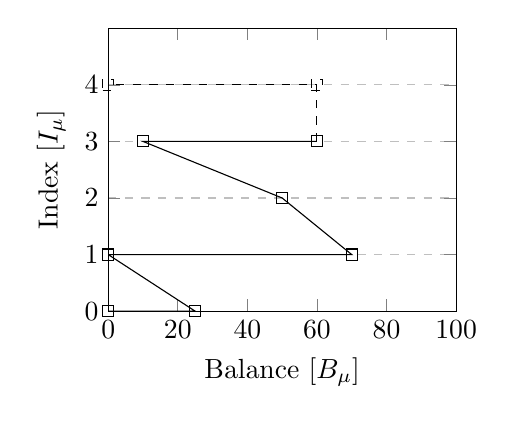
\begin{tikzpicture}
    \begin{axis}[
        xlabel={Balance [$B_\mu$]},
        ylabel={Index [$I_\mu$]},
        xmin=0, xmax=100,
        ymin=0, ymax=5,
        xtick={0,20,40,60,80,100},
        ytick={0,1,2,3,4},
        ymajorgrids=true,
        grid style=dashed,
    ]

    \addplot[
        color=black,
        mark=square,
        ]
        coordinates {
            (0,0)(25,0)(0,1)(70,1)(50,2)(10,3)(60,3)
        };

    \addplot[
        color=black,
        mark=square,
        dashed,
        ]
        coordinates {
            (60,3)(60,4)(0,4)
        };

    \end{axis}
    \end{tikzpicture}}
\subfloat[$(I_\mu,B_\mu,R_\mathcal{P}) \rightarrow (I_\mu+1, B_\mu\uparrow,R_\mathcal{P})$]{
    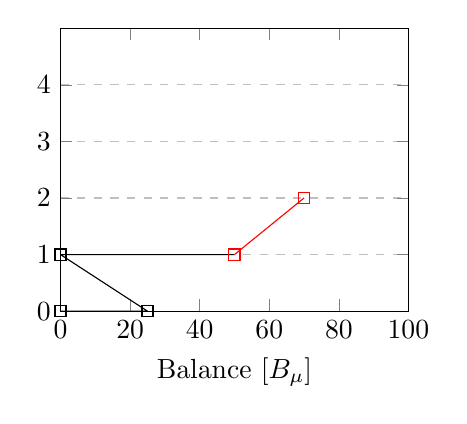
\begin{tikzpicture}
    \begin{axis}[
        xlabel={Balance [$B_\mu$]},
        xmin=0, xmax=100,
        ymin=0, ymax=5,
        xtick={0,20,40,60,80,100},
        ytick={0,1,2,3,4},
        ymajorgrids=true,
        grid style=dashed,
    ]

    \addplot[
        color=black,
        mark=square,
        ]
        coordinates {
            (0,0)(25,0)(0,1)(50,1)
        };

    \addplot[
        color=red,
        mark=square,
        ]
        coordinates {
            (50,1)(70,2)
        };

    \end{axis}
    \end{tikzpicture}}\\
\subfloat[$(I_\mu, B_\mu,R_\mathcal{P}) \rightarrow (I_\mu\downarrow,\_,R_\mathcal{P})$]{
    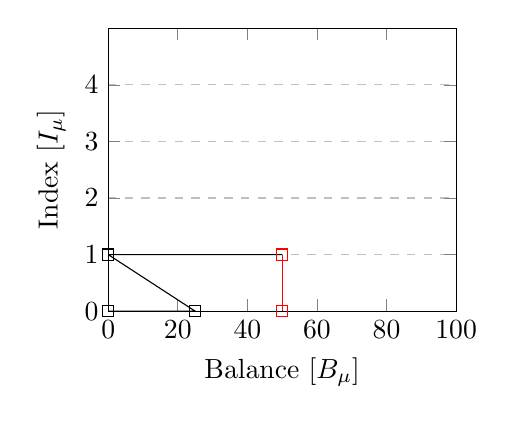
\begin{tikzpicture}
    \begin{axis}[
        xlabel={Balance [$B_\mu$]},
        ylabel={Index [$I_\mu$]},
        xmin=0, xmax=100,
        ymin=0, ymax=5,
        xtick={0,20,40,60,80,100},
        ytick={0,1,2,3,4},
        ymajorgrids=true,
        grid style=dashed,
    ]

    \addplot[
        color=black,
        mark=square,
        ]
        coordinates {
            (0,0)(25,0)(0,1)(50,1)
        };

    \addplot[
        color=red,
        mark=square,
        ]
        coordinates {
            (50,1)(50,0)
        };

    \end{axis}
    \end{tikzpicture}}
\subfloat[$(I_\mu,B_\mu,R_\mathcal{P}) \rightarrow (I_\mu, B_\mu\downarrow,R_\mathcal{P})$]{
    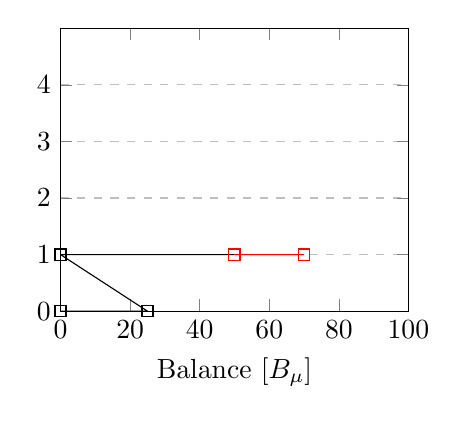
\begin{tikzpicture}
    \begin{axis}[
        xlabel={Balance [$B_\mu$]},
        xmin=0, xmax=100,
        ymin=0, ymax=5,
        xtick={0,20,40,60,80,100},
        ytick={0,1,2,3,4},
        ymajorgrids=true,
        grid style=dashed,
    ]

    \addplot[
        color=black,
        mark=square,
        ]
        coordinates {
            (0,0)(25,0)(0,1)(70,1)
        };

    \addplot[
        color=red,
        mark=square,
        ]
        coordinates {
            (70,1)(50,1)
        };

    \end{axis}
    \end{tikzpicture}}
\caption{State transitions in $M$, transitions in red are not allowed. Dashed transition are during refund process. The first step is the refund request, the second can be either claim, resolve, or dispute. Figure (c) show validity index decrementation, this is invalid no matter of the resulting balance amount. Figure (d) shows a decreasing balance, red line owerflow the black line.}
\label{fig:contractStateTransitions}
\end{figure}

\subsection{Channel state, $\sigma \rightarrow \sigma'$} Channel state transitions ($\sigma \xrightarrow{\delta_\sigma \lor \mu \rightarrow \mu'} \sigma'$) are triggered by delta changes $\delta_\sigma \in \Delta$ or by transitions in $M$, i.e. $\mu \rightarrow \mu'$. The base channel state $\sigma$ is computed as
\begin{equation*}
\begin{split}
  \sigma &=
  \begin{cases}
    \emptyset & \quad \text{if no previous state exists} \\
      (I_\sigma, B_\sigma, D, S, R) & \quad \text{otherwise}
  \end{cases}
\end{split}
\end{equation*}

\subsubsection{Payment, $\delta_\sigma(a)$.} Payments trigger transition in channel states from the base state $\sigma$ to a destination state $\sigma'$ noted $\sigma \xrightarrow{\delta_\sigma(a)} \sigma'$.
The destination channel state is computed as
\begin{equation*}
\begin{split}
  \sigma' &=
  \begin{cases}
      \emptyset & \quad \text{if } \sigma = \emptyset \\
      (I_\mu, B_\mu, D, S+a, R) & \quad \text{otherwise}
  \end{cases}
\end{split}
\end{equation*}

Payments cannot be accepted without a previous state. If $\sigma = \emptyset$ then the channel is not initialized yet and must not accept any payments.

\subsubsection{Top up, $\mu \xrightarrow{\delta_\mu(a)} \mu'$.} Each top up event modify the contract state $\mu$, then the channel state $\sigma$ must be updated to keep track of the real balance. The destination channel state is computed as \begin{equation*}
\begin{split}
  \sigma' &=
  \begin{cases}
      (0, B_\mu, B_\mu, 0, 0) & \quad \text{if } \sigma = \emptyset \\
      (I_\sigma, B_\mu, D + B_\mu - B_\sigma, S, R) & \quad \text{otherwise}
  \end{cases}
\end{split}
\end{equation*}

where
$$B_\mu - B_\sigma = a$$

It is worth noting that if no previous state exists the channel is initialized and the first state is created.

\subsubsection{Settle, $\mu \xrightarrow{\sigma''} \mu'$.} Settlements trigger transition in contract state $\mu \rightarrow \mu'$ and then the channel state $\sigma$ must be updated as
\begin{equation*}
\begin{split}
  \sigma' &=
  \begin{cases}
      \emptyset & \quad \text{if } \sigma = \emptyset \\
      (I_\mu, B_\mu, D, S, R) & \quad \text{otherwise}
  \end{cases}
\end{split}
\end{equation*}

\subsubsection{Refund, $\mu \xrightarrow{\sigma''} \mu'\ |\ R_\mathcal{P} \geq 0$.} Clients can ask for refund and modify the contract state then the channel state must be updated as
\begin{equation*}
\begin{split}
  \sigma' &=
  \begin{cases}
      \emptyset & \quad \text{if } \sigma = \emptyset \\
      (I_\mu, B_\sigma, D, S, R) & \quad \text{otherwise}
  \end{cases}
\end{split}
\end{equation*}

and the state of the channel must enter is ``refund mode'' until the refund is ended with either a dispute, resolve, or a claim. During this periode client must not send new payments to prevent the provider to successfully dispute the refund (even if updating the channel state to $I_\sigma = I_\mu$ normlay prevent negociating payment for $I_m = I_\mu$).

\subsubsection{Dispute, $\mu \xrightarrow{\sigma''} \mu'$.} When request refunds are resolved with a dispute the provider can take what he owns during the dispute plus some penalties $\rho$.

\begin{equation*}
\begin{split}
  \sigma' &=
  \begin{cases}
      \emptyset & \quad \text{if } \sigma = \emptyset \\
      (I_\sigma, B_\mu, D, S + \rho, B_\mu - R_\mathcal{P} - \rho) & \quad \text{otherwise}
  \end{cases}
\end{split}
\end{equation*}

such that
$$D = S + R \land B_\mu = 0$$

\subsubsection{Resolve \& Claim, $\mu \xrightarrow{\sigma''} \mu'$.} Provider can accept the request and resolve a refund request by submitting the settle directive $d_s$ or a client can claim his funds after the delay. In both cases the contract state $\mu$ changes, then the channel state must be updated as
\begin{equation*}
\begin{split}
  \sigma' &=
  \begin{cases}
      \emptyset & \quad \text{if } \sigma = \emptyset \\
      (I_\sigma, B_\mu, D, S, B_\mu - R_\mathcal{P}) & \quad \text{otherwise}
  \end{cases}
\end{split}
\end{equation*}

such that
$$D = S + R \land B_\mu = 0$$

\begin{table}[t]
  \begin{tabularx}{\textwidth}{| S | S | C | C | C |}
    \cline{2-5}
      \multicolumn{1}{c|}{ } & $\delta$ & $\mu$ & $m$ & $\sigma$ \\ \cline{2-5}
      \multicolumn{1}{c|}{ } & $\delta(a)$ & $(I_\mu,B_\mu,R_\mathcal{P})$ & $(I_m,B_\sigma,D_m,S)$ & $(I_\sigma,B_\sigma,D,S,R)$ \\
  \hhline{~====}
      \multicolumn{1}{c|}{ } & & $(0,0,0)$ & & $\emptyset$ \\ \cline{1-1}
      top up  & $\delta_\mu(10)$   & $(0,10,0)$ &               & $(0,10,10,0,0)$ \\
      payment & $\delta_\sigma(1)$ &            & $(1,10,10,1)$ & $(0,10,10,1,0)$ \\
      payment & $\delta_\sigma(1)$ &            & $(1,10,10,2)$ & $(0,10,10,2,0)$ \\
      settle  &                    & $(1,8,0)$  &               & $(1,8,10,2,0)$ \\
      payment & $\delta_\sigma(2)$ &            & $(2,8,10,4)$  & $(1,8,10,4,0)$ \\
      payment & $\delta_\sigma(2)$ &            & $(2,8,10,6)$  & $(1,8,10,6,0)$ \\
      top up  & $\delta_\mu(10)$   & $(1,18,0)$ &               & $(1,18,20,6,0)$ \\
      payment & $\delta_\sigma(1)$ &            & $(2,18,20,7)$ & $(1,18,20,7,0)$ \\
      settle  &                    & $(2,13,0)$ & $(3,13,20,7)$ & $(2,13,20,7,0)$ \\
      refund  &                    & $(3,13,0)$ &               & $(3,13,20,7,0)$ \\
      claim   &                    & $(3,0,0)$  &               & $(3,0,20,7,13)$ \\
      \cline{1-5}
  \end{tabularx}
  \medskip
  \caption{State transitions during channel lifetime}
\end{table}

\begin{table}[t]
  \begin{tabularx}{\textwidth}{| S | S | C | C | C |}
    \cline{2-5}
      \multicolumn{1}{c|}{ } & $\delta$ & $\mu$ & $m$ & $\sigma$ \\ \cline{2-5}
      \multicolumn{1}{c|}{ } & $\delta(a)$ & $(I_\mu,B_\mu,R_\mathcal{P})$ & $(I_m,B_\sigma,D_m,S)$ & $(I_\sigma,B_\sigma,D,S,R)$ \\
  \hhline{~====}
      \multicolumn{1}{c|}{ } & & $(0,0,0)$ & & $\emptyset$ \\ \cline{1-1}
      top up  & $\delta_\mu(3)$    & $(0,3,0)$  &                & $(0,3,3,0,0)$ \\
      top up  & $\delta_\mu(2)$    & $(0,5,0)$  &                & $(0,5,5,0,0)$ \\
      payment & $\delta_\sigma(3)$ &            & $(1,5,5,3)$    & $(0,5,5,3,0)$ \\
      settle  &                    & $(1,2,0)$  &                & $(1,2,5,3,0)$ \\
      payment & $\delta_\sigma(1)$ &            & $(2,2,5,4)$    & $(1,2,5,4,0)$ \\
      top up  & $\delta_\mu(2)$    & $(1,4,0)$  &                & $(1,4,7,4,0)$ \\
      settle  &                    & $(2,3,0)$  &                & $(2,3,7,4,0)$ \\
      payment & $\delta_\sigma(2)$ &            & $(3,3,7,6)$    & $(2,3,7,6,0)$ \\
      refund  &                    & $(3,3,2)$  &                & $(3,3,7,6,0)$ \\
      top up  & $\delta_\mu(10)$   & $(3,13,2)$ &                & $(3,13,17,6,0)$ \\
      resolve &                    & $(3,0,0)$  &                & $(3,0,17,6,11)$ \\
      top up  & $\delta_\mu(15)$   & $(3,15,0)$ &                & $(3,15,32,6,11)$ \\
      payment & $\delta_\sigma(7)$ &            & $(4,15,21,13)$ & $(3,15,32,13,11)$ \\
      payment & $\delta_\sigma(5)$ &            & $(4,15,21,18)$ & $(3,15,32,18,11)$ \\
      top up  & $\delta_\mu(3)$    & $(3,18,0)$ &                & $(3,15,35,18,11)$ \\
      settle  &                    & $(4,6,0)$  &                & $(4,6,35,18,11)$ \\
      \cline{1-5}
  \end{tabularx}
  \medskip
  \caption{Settlement after top up and refund resolved}
\end{table}

\section{Protocol} The protocol describes interactions between clients and the provider and message negotiation. Protocol defines the derivation of directives from messages.

\subsubsection{Client actions} A client can send money through the channel and refund his money after some time if he submitted the right message $m$ corresponding to the latest channel state $\sigma$.

\subsubsection{Provider actions} The provider can settle channels with his latest message corresponding to the latest channel state. If a client requests a refund, the provider has the choice to dispute it or resolve it.

\subsubsection{Anyone actions} Anyone can top up a channel for himself or for another client.

\subsection{Payment, $\delta_\sigma(a)$} Payments are negotiated with of one acquire directive for the provider signed by the client.

\subsubsection{Settle directive, $d_s$} Settle directive $d_s$ allows the provider to claim immediately, i.e. without any delay, his owned amount for a specific channel. The client must not be able to apply a settle directive on behalf of the provider.
\begin{equation*}
\begin{split}
    h &= \texttt{keccak256}(\texttt{contract},c,I_m,B_\sigma,D_m,S) \\
    d_s &= \texttt{sign}(\texttt{prefix}, h) \quad \text{with $c$ private key} \\
\end{split}
\end{equation*}

\subsection{Refund} Opening a refund is performed with one directive self-generated by the client and signed by himself. The provider must not be able to create directives $d_r$ nor apply a refund directive on behalf of the client.

\subsubsection{Refund directive, $d_r$} Refund directive $d_r$ allows the client to claim all the remaining funds and transfer them after some delay if the provider is not able to dispute the claim nor resolves the request. The provider is not able to dispute the claim if the directive is generated from the message derived by the latest channel state in $\Sigma$.
\begin{equation*}
\begin{split}
    h &= \texttt{keccak256}(\texttt{contract},c,I_m,O(\mathcal{P})) \\
    d_r &= \texttt{sign}(\texttt{prefix}, h) \quad \text{with $c$ private key} \\
\end{split}
\end{equation*}

with
\begin{equation*}
\begin{split}
    O(\mathcal{P}) &= B_\mu - A \\
    &= B_\mu - (D_m - S + B_\mu - B_\sigma) \\
\end{split}
\end{equation*}

A refund request can be closed in three different manners
\begin{equation*}
\begin{split}
    \text{close a refund by}
  \begin{cases}
      \text{dispute} & \quad \text{if the provider is able to prove a lie} \\
      \text{resolve} & \quad \text{if the provider agrees} \\
      \text{claim} & \quad \text{otherwise by the client after delay} \\
  \end{cases}
\end{split}
\end{equation*}

\subsection{Dispute refund} Disputes are won if the provider can prove that is owns a payment directive $d_s$, i.e. client agreed on a later channel state $\sigma'$, where
$$O(\mathcal{P})' > O(\mathcal{P}), \quad O(\mathcal{P})' \in d_s \land O(\mathcal{P}) \in d_r$$

with
\begin{equation*}
\begin{split}
    O(\mathcal{P})' &= B_\mu - A \\
    &= B_\mu - (D_m - S + B_\mu - B_\sigma) \\
\end{split}
\end{equation*}

\subsection{Resolve refund} Provider can choose to agree with the request and resolve it directly. By resolving the request the provider will get his remaining funds and send the client available funds $A$ directly to the client. It is worth noting that the provider has no incentive to resolve requests where $S = 0$.

\subsection{Claim refund} The client can claim his funds after the delay if the provider has not disputed nor resolved the request.

\section{Sub-channel applications} In this chapter we describe how to use sub-channels to build a partially trusted pre-authorized payment layer. Pre-authorized payments in sub-channel $\omega_p$ can be merged at any moment into the main channel $\omega$ given a partially-trusted model.

\subsubsection{Partially-trusted pre-authorized payments model} We define in this model of pre-authorized payments the amount of trust required by the client in favour of the provider. We define the trust as

\begin{quote}
    At any time the client puts at risk at most a pre-authorization of $l$ amount and trusts the provider to take $x \leq l$ amount only when necessary. Client can never loose more than $l$ in the case of a provider misbehaving.
\end{quote}

\subsection{Pre-authorized payments sub-channel} We first define a unique sub-channel $\omega_p$ per client that allows the provider at any moment to take an arbitrary amount $x \leq l$ up to a limit $l$ set by the client. The sub-channel must follow the partially-trusted model defined previously. The client must be able to increase the limit $l$ and merge an arbitrary amount $y \leq l$ at any moment into the main channel $\omega$.

%The rules for this sub-channel are defined by the following: (i) at any moment the client risks at most $l$, (ii) $l$ can be increased instantly with cooperation between client and provider, (iii) $l$ can be decreased by $x$ instantly with cooperation if the main channel $\omega$ is increased by $x$, and (iv) $l$ can be decreased without cooperation by the client with some delay.

Sub-channel $\omega_p$ is composed of a sub-channel state $\Sigma^p$ and contract state $M^p \subset M$. Sub-channel states are noted $\sigma^p \in \Sigma^p$. We define an increase of the limit $l$ as $\delta_{\sigma^p}$. The transition between two sub-channel states can be triggered with a delta or because of a merge into the main channel.

We redefine the transition condition for contract states as
$$\mu \xrightarrow{\delta_\mu \lor \sigma \lor \sigma^p} \mu'$$

the redefinition of transition condition for main channel states as
$$\sigma \xrightarrow{\delta_\sigma \lor \sigma^p \lor \mu \rightarrow \mu'} \sigma'$$

and the new transition condition for sub-channel states as
$$\sigma^p \xrightarrow{\delta_{\sigma^p} \lor \sigma \xrightarrow{\sigma^p} \sigma'} \sigma^{\prime p}$$

We also define the new transition rules as
\begin{equation*}
\begin{split}
    \mu \xrightarrow{\sigma^p} \mu' &: \quad \mu' = \mu \cup \sigma^p = \mu \cup \{ \delta_{\sigma^p} \} \\
    \sigma \xrightarrow{\sigma^p} \sigma' &: \quad \sigma' = \sigma \cup \sigma^p = \sigma \cup \{ \delta_{\sigma^p} \} \\
    %\sigma \xrightarrow{\delta_{\sigma^p}} \sigma' &: \quad \sigma' = \sigma \cup \{ \delta_{\sigma^p} \}  \\
    \sigma \xrightarrow{\mu \xrightarrow{\sigma^p} \mu'} \sigma' &: \quad \sigma' =  \sigma \cup \mu' = \sigma \cup \{ \delta_{\sigma^p} \} \\
\end{split}
\end{equation*}

It is worth noting that sub-channel states can be enforced directly on the contract layer or merged into the main channel state, but in both case the main channel state is updated accordingly. We miss two more rule definitions
\begin{equation*}
\begin{split}
    \sigma^p \xrightarrow{\delta_{\sigma^p}} \sigma^{\prime p} &: \quad \sigma^{\prime p} = \sigma^p \cup \{ \delta_{\sigma^p} \} \\
    \sigma^p \xrightarrow{\sigma \xrightarrow{\sigma^{\prime\prime p}} \sigma'} \sigma^{\prime p} &: \quad \sigma^{\prime p} = \sigma^p \setminus \sigma^{\prime\prime p} \\
\end{split}
\end{equation*}

When a sub-channel state is merged into the main channel state, the sub-channel deltas are moved into the state channel and removed from the sub-channel.

\subsubsection{Sub-channel merge} Sub-channel merges move the total limit $l$ (sum of all deltas in sub-channel state) into the main channel and can be defined as
\begin{equation*}
\begin{split}
    \Sigma^p&: \sigma_1^p \xrightarrow{\sigma_1 \xrightarrow{\sigma_1^p} \sigma_2} \sigma_2^p \\
    \Sigma&: \sigma_1 \xrightarrow{\sigma_1^p} \sigma_2 \\
\end{split}
\end{equation*}

where $\sigma_2$ contains all deltas, i.e. the total limit $l$. Set's states can be computed with the previous rules given the base states $\sigma^p_1$ and $\sigma_1$ as
\begin{align*}
    \sigma^p_1 &= \{\delta_{\sigma^p}\} \\
    \sigma_1   &= \{\delta_\sigma\} \\
    \sigma_2   &= \{\delta_\sigma\} \cup \{\delta_{\sigma^p}\} & &= \{\delta_\sigma,\delta_{\sigma^p}\} \\
    \sigma^p_2 &= \{\delta_{\sigma^p}\} \setminus \{\delta_\sigma,\delta_{\sigma^p}\} & &= \emptyset
\end{align*}

We say that the main channel state contains a sub-channel state if the sub-channel state has been merged. The rule follows the superset rule
$$\sigma \supset \sigma^p \iff \exists \sigma' \mid \sigma' \xrightarrow{\sigma^p} \sigma$$

\paragraph{Channels' states pairings} We define pairings of main channel and sub-channel states. States in pairings can be either non-exclusive $\parallel$, i.e. both states can be enforced on the contract layer, or mutually exclusive $\perp$, i.e. only one of the two states can be enforced.

We define, as previously shown, four states when a merge happens: $\sigma_1, \sigma_2, \sigma^p_1, \sigma^p_2$. We define three pairings of states (noted $1, 2, 3$) with only one state in channel and sub-channel as
\begin{equation*}
    \begin{matrix}
        \sigma^p_1 & \xrightarrow{\sigma_1 \xrightarrow{\sigma^p_1} \sigma_2} & \sigma^p_2 \\
        \vdots_1 & \ddots_2 & \vdots_3 \\
        \sigma_1 & \xrightarrow{\sigma^p_1} & \sigma_2 \\
    \end{matrix}
\end{equation*}

To guarantee the partially-trusted model the pairing 1 is non-exclusive and must be valid at any moment but must invalidate the pairing 3. The inverse is also true. The pairing 2 must be mutually exclusive, e.g. if $\sigma^p_1$ is enforced then $\sigma_2 : \sigma_2 \supset \sigma^p_1$ must be invalid in the contract layer. Otherwise deltas in $\sigma^p_1$ can be used twice and the partialy-trusted model is broken.

Given the previous case we can derive generic rules
$$\forall (\sigma, \sigma^p) : \sigma \perp \sigma^p \iff \sigma \supset \sigma^p$$

and
$$\forall (\sigma, \sigma^p) : \sigma \parallel \sigma^p \iff \sigma \not \supset \sigma^p$$

The fourth pairing $(\sigma_1, \sigma^p_2)$ is valid but does not represent a threat for the clients. Deltas merged in $\sigma_2$ are removed in $\sigma^p_2$ because of the rule
$$\sigma^p \xrightarrow{\sigma \xrightarrow{\sigma^{\prime\prime p}} \sigma'} \sigma^{\prime p} : \quad \sigma^{\prime p} = \sigma^p \setminus \sigma^{\prime\prime p}$$

and are not in $\sigma_1$. So $\sigma_1 + \sigma^p_2$ have less value than the three other pairings. It is worth noting that the pairing 3 $(\sigma_2, \sigma^p_2)$ is equal to $(\sigma_2, \emptyset)$ and then is the same as only enforced $\sigma_2$.

\subsubsection{Sub-channel partial merge} Sub-channel partial merges move an arbitrary amount $y < l$ into the main channel and can be defined as
\begin{align*}
    \Sigma^p&: \sigma_1^p \xrightarrow{\sigma_1 \xrightarrow{\sigma_1^p} \sigma_2} \sigma_2^p \xrightarrow{\delta^\prime_{\sigma^p}} \sigma_3^p & &\mid l(\delta^\prime_{\sigma^p}) = l - y \\
    \Sigma&: \sigma_1 \xrightarrow{\sigma_1^p} \sigma_2 & &\mid y(\sigma_1^p) < l
\end{align*}

where initial limit $l = \sigma^p_1$ and $\sigma^p_1 \perp \sigma_2 \land \sigma^p_3 \parallel \sigma_2$. The security of a partial merge inherits the security of a merge only if the value of pairing $(\sigma_2, \sigma^p_3)$ is greater than or equal to pairing $(\sigma_1, \sigma^p_1)$.

\begin{table}[t]
  \begin{tabularx}{\textwidth}{| S | C | C | C |}
    \cline{2-4}
      \multicolumn{1}{c|}{ } & $\mu$ & $\sigma$ & $\sigma^p$ \\ \cline{2-4}
      \multicolumn{1}{c|}{ } & $(I_\mu,I_{\mu^p},N_\mu,B_\mu,R_\mathcal{P})$ & $(I_\sigma,N_\sigma,B_\sigma,D,S,R)$ & $(I_{\sigma^p},N_{\sigma^p},L)$ \\
  \hhline{~===}
      \multicolumn{1}{c|}{ } & $\mu_0(0,0,0,0,0)$  & $\emptyset$          & $\emptyset$ \\ \cline{1-1}
      $\delta_\mu^{10}$      & $\mu_1(0,0,0,10,0)$ & $\sigma_1(0,0,10,10,0,0)$    &             \\
      $\delta_{\sigma^p}^3$  &                &                      & $\sigma^p_1(0,0,3)$   \\
      $\delta_\sigma^4$ &    & $\sigma_2(0,0,10,10,4,0)$  & \\
      $\delta_\sigma^1 + \delta_{\sigma^p}^2$ & & $\sigma_3(0,1,10,10,5,0)$  & $\sigma^p_2(0,1,2)$   \\
      $\delta_{\sigma^p}^3$  &                &                      & $\sigma^p_3(0,1,5)$   \\
      \cline{1-4}
      \multicolumn{4}{c}{ $\cdots$ } \\
      \cline{1-4}
      $\sigma^p_1(\mu_1)^3$ & $\mu_2(0,1,0,7,0)$ & $\sigma_3(0,0,7,10,7,0)$ & \\
      $\sigma_2(\mu_2)^3$ & $\mu_3(1,1,0,3,0)$ & $\sigma_4(1,0,3,10,7,0)$ & \\
      \cline{1-4}
      \multicolumn{4}{c}{ $\cdots$ } \\
      \cline{1-4}
      $\sigma_3(\mu_1)$ & $\mu_2(1,0,1,5,0)$ & $\sigma_4(1,0,5,10,5,0)$ & \\
      $\sigma^p_3(\mu_2)^2$ & $\mu_3(1,1,1,3,0)$ & $\sigma_5(1,1,3,10,7,0)$ & \\
      \cline{1-4}
      \multicolumn{4}{c}{ $\cdots$ } \\
      \cline{1-4}
      $\sigma^p_3(\mu_1)^2$ & $\mu_2(0,1,1,8,0)$ & $\sigma_4(0,1,8,10,7,0)$ & \\
      $\sigma_3(\mu_2)$ & $\mu_3(1,1,1,3,0)$ & $\sigma_4(1,1,3,10,7,0)$ & \\
      \cline{1-4}
  \end{tabularx}
  \medskip
    \caption{State transitions with a sub-channel $\omega_p$}
\end{table}

\subsection{Contract state}

\subsection{Contract state transition} Validity rules of indexes $N$ and $I$ are defined as follows
%$$N_\mu < N_\sigma \quad\quad\quad  N_{\mu} < N_{\sigma^p}$$
%$$N_\mu < N_\sigma < N_{\sigma^p}$$

and
$$I_\mu = I_\sigma \quad\quad\quad  I_{\mu^p} = I_{\sigma^p}$$

%\begin{equation*}
%\begin{split}
%    \Sigma^p&: \emptyset \xrightarrow{\delta_{\sigma^p}} \sigma_1^p \xrightarrow{\sigma_1 \xrightarrow{\sigma_1^p} \sigma_2} \sigma_2^p \xrightarrow{\delta^\prime_{\sigma^p}} \sigma_3^p \\
%    \Sigma&: \emptyset \xrightarrow{\emptyset \xrightarrow{\delta_\mu} \mu_1} \sigma_1 \xrightarrow{\sigma_1^p} \sigma_2 \\
%    M&: \emptyset \xrightarrow{\delta_\mu} \mu_1 \\
%\end{split}
%\end{equation*}

%\section{Acknowledgement} Loan Ventura, Thomas Roulin and Nicolas Huguenin are acknowledged for their helpful contribution and comments during the completion of this work.

%
% ---- Bibliography ----
%
\printbibliography

\end{document}
